%%%%%%%%%%%%%%%%%%%%%%%%%%%%%%%%%%%%%%%%%
%% Author        : @PrakashGautam      %%
%% Date Written	 : December 30, 2014   %%
%% Last Updated  : August 16, 2015     %%
%% Editor Used   : gVim v 7.30         %% 
%%%%%%%%%%%%%%%%%%%%%%%%%%%%%%%%%%%%%%%%%
\documentclass[a4paper,12pt]{article}
\usepackage[top=35mm,left=35mm,bottom=20mm,right=20mm]{geometry}
\usepackage{fontspec}
\setmainfont{Times New Roman}
%
%
\usepackage{epstopdf}
\usepackage{graphicx}
\usepackage{pstricks}
\usepackage{tikz}
\usepackage{circuitikz}
\usepackage{pgfgantt}
\usepackage{hyperref}
\hypersetup{colorlinks = false}
\hypersetup{pdfborder = {0 0 0}}
\graphicspath{Images/}
%
\usepackage{listings}
%
\makeatletter
	\def\input@path{{include/}}
\makeatother
%

\parskip=1\baselineskip
\parindent = 0pt 
%
\usepackage{titlesec,titleps}
%
\titleformat{\section}[hang]{\bfseries\large}{\thesection.}{1em}{\MakeUppercase}
\titlespacing*{\section}{0pt}{1\baselineskip}{1\baselineskip}
%
\titleformat{\subsection}[hang]{\bfseries}{\thesubsection}{1em}{}
\titlespacing*{\subsection}{0pt}{1\baselineskip}{1\baselineskip}
%
\renewpagestyle{plain}{%
	\sethead{}{\itshape\sectiontitle}{\thepage}
	\setfoot{}{}{}
}
%
\renewcommand{\baselinestretch}{1.5} 


\usepackage[acronym,nomain]{glossaries} 
%
\makeglossaries
\input{ListingColour.tex}%
\newacronym{pcb}{PCB}{Printed Circuit Board}
\newacronym{led}{LED}{Light Emitting Diode}
\newacronym{irled}{IRLED}{Infra-Red Light Emitting Diode}
\newacronym{gps}{GPS}{Global Positioning System}
\newacronym{rtls}{RTLS}{Real Time Location System}
\newacronym{lps}{LPS}{Local Positioning System}
\newacronym{rfid}{RFID}{Radio Frequency Identitification}
\newacronym{ir}{IR}{Infrared}
\newacronym{rf}{RF}{Radio Frequency}
\newacronym{wlan}{WLAN}{Wireless Local Area Network}
\newacronym{uwb}{UWB}{Ultra Wide Band}
\newacronym{gui}{GUI}{Graphical User Interface}
\newacronym{toa}{TOA}{Time of Arrival}
\newacronym{tof}{TOF}{Time of Flight}
\newacronym{aoa}{AOA}{Angle of Arrival}
\newacronym{ic}{IC}{Integrated Circuit}
\newacronym{id}{ID}{Identity}
\newacronym{tv}{TV}{Television}
\newacronym{dc}{DC}{Direct Current}
\newacronym{risc}{RISC}{Reduced Instruction Set Computer}
\newacronym{pwm}{PWM}{Pulse Width Modulation}
\newacronym{cmrr}{CMRR}{Common Mode Rejection Ratio}
\newacronym{api}{API}{Application Programming Interface}
\newacronym{spi}{SPI}{Serial Peripheral Interface}
\newacronym{usb}{USB}{Universal Serial Bus}
%
%
%
%
\begin{document}%
%
%
\begin{titlepage}
	\begin{center}
		\begin{Huge}
			Tribhuvan University\\
%			\includegraphics[scale=1]{logo.png}\\
			Institute of Engineering\\
			 Pulchowk Campus\\
		\end{Huge}
			Pulchowk Lalitpur,Nepal.\\
			\vfill
		\textbf{
					A\\
					Mid-Term Report on\\
					Major Project\\
					(Real Time Location System(RTLS) based\\
					License Trial Automation System)\\
				}
		\vfill

		\textbf{Submitted To:\\}
			Department of Electronics and Computer Engineering\\[2cm]
		\textbf{Submitted by:\\}
			Prajjwal Raj Kandel (068BEX428)\\
			Prakash Gautam (068BEX429)\\
			Sudip Prasai (068BEX442)\\
			Utsav Bhetwal (068BEX447)\\
			\vfill
			August 18, 2015
	\end{center}
\end{titlepage}

%%
\pagenumbering{roman}

\begin{center}
	\begin{Large}
		\textbf{Approval Sheet}\\[1cm]
	\end{Large}
	\vfill
	TRIBHUVAN UNIVERSITY\\
	INSTITUTE OF ENGINEERING\\
	PULCHOWK CAMPUS\\
	DEPARTMENT OF ELECTRONICS AND COMPUTER ENGINEERING\\
\end{center}
The undersigned certify that they have read, and recommended to the Institute of Engineering for acceptance, a project report entitled \emph{"RTLS Based License Trial Automation System"}  submitted by Prajjwal Raj Kandel (068BE428), Prakash Gautam (068BEX429), Sudip Prasai(068BEX442) and Utsav Bhetwal(068BEX447), in partial fulfilment of the requirements for the Bachelor’s degree in Electronics and Communication Engineering.
%\vfill

--------------------------------------------------------\\
Project Supervisor, 
Mr. Tika Upreti\\
Associate Professor \\
Department of Electronics 
and Computer Engineering \\
Central Campus,
Institute Of Engineering \\
\\
--------------------------------------------------------\\
Internal Examiner, 
Dr. Jyoti Tandukar \\
Associate Professor \\
Department of Electronics 
and Computer Engineering \\
Central Campus,
Institute Of Engineering \\
\\
--------------------------------------------------------\\
External Examiner, 
Mr. Shanta Maharjan \\
Associate Professor\\
Department of Electronics 
and Computer Engineering \\
Thapathali Campus,
Institute Of Engineering \\
\textbf{Approved on \today}
%
\section*{Preface}
Nepal Government has introduced a new trial system for providing license to drivers. Traffic authorities present at the trial venue decide on the basis of inspection whether the driver is qualified to acquire a driving license or not.

Use of technology in the field of road traffic management has long prevalence in Nepal, specially though the use of automatic traffic lights placed at almost every chowks of the cities with busy traffic. Use of breathalyzers to control the drink-drive cases in Nepal has had a great positive impact reducing significantly the road accidents. This has eased the task of policeman as well as increased human safety. 


Also the use of radar gun to measure the vehicle speed on road has assisted the police greatly instantly capturing a overspeed vehicle thereby preventing a potential accident. 


Use of technology has clearly have a positive impact in the traffic management area. One area that still lacks proper use of technology is traffic license acquiring process by riders and drivers. So far in Nepal the rider is let drive on the specially designed track to decide whether he is capable enough to drive safely in the busy road. Human invigilator inspects the whole process.But human eye inspection is not reliable enough to decide, with great accuracy the prevalent license trial system.


Articles in newspapers suggest that the increased road accidents are directly related to the drivers driving their vehicle without acquiring license or those acquiring fraud license without passing the trial examination.


Though the new trial system improves the standard of examination and tests the drivers properly, rumors of people acquiring fraud driving license do not cease to exist. Thus the idea is to build a system where a computer rather than human eye decides the validity of a trial, thus eliminating the chances of fraud license.



%
\newpage	
%
\section*{Acknowledgement}
We would extend our sincere gratitude the department of Electronics and Communication Engineering, Pulchowk Campus, for encouraging us to work on this project. We would also like to thank the department for providing us with a project room facilitated with an oscilloscope and function generator which really helped us to proceed in the project.

We would also like to thank our project supervisor Associate Professor Tika Upreti for encouraging us to complete the project and for providing us with his invalueable suggestions. Also we would like to thank all our friends without whose support this project would not have been possible.


%
\newpage
%
\begin{abstract}
For the fulfillment of course requirement for Electronics Engineering student are required to do a project with considerable level of difficulty applying the theoretical knowledge acquired during the whole tenure of undergraduate studies. This is final report of the project. We have chosen to do a project in \gls{rtls}, based license trial automation system to improve the existing trial system in Nepal. We have first proposed this system to be applied for the trial automation for two-Wheeler motorbikes. In first phase, ultrasonic sensors are used to find the distance of the vehicle form  at least three predefined locations, then use trilateration to find the exact space co-ordinate referring to our local coordinate system. We have used ultrasonic sensors to find the distance of the object from three predefined locations. The next phase is to apply the positioning system to automate the trial system. There is a provision of graphical visualization of the process in an \gls{gui} application.
\end{abstract}

%
\newpage
%
\tableofcontents
%
\newpage
%
\listoffigures
\listoftables
%
\newpage
%
\printglossaries
%
\newpage
\pagenumbering{arabic}
%
%
\newpage
%\printacronyms[include-classes=abbrev,name=Abbreviations]
%
\section{Introduction}
The need to locate people and objects as soon as possible has always been an important part of any organization or industry. With use of wireless technology, we are trying to remotely locate objects within a predefined time frame. \gls{gps} is obviously the most widely used outdoor location sensing technology, but there are several drawbacks which make \gls{gps} impossible to be used as an indoor positioning system with high precision. Due to line-of-sight demand between the satellites and the receiver, and specialized hardware requirement, it has poor indoor coverage and insufficient accuracy\cite{Insufficient}. 

We typically use small low-power transceiver attached to assets as well as sets of readers that map the location of these assets. Systems that map a location relative to a fixed set of coordinates are more accurately called \gls{rtls}. Wireless \gls{rtls} tags are attached to objects or worn by people, and in most \gls{rtls}, fixed reference points receive wireless signals from tags to determine their location. \gls{rtls} is one of the latest solutions for tracking objects in real time with high precision. \gls{rtls} has many advantages and can be combined with different technologies depending in which it is being applied. This is the type of system that we are looking to build first and implement it to automate the driving license trial system.


\subsection{Objectives}
The major objectives behind trying to build this system is to replace traditional human inspection based method of giving license to the drivers in the license trial.  
\begin{enumerate}
\item To fulfill the course requirement.
\item To apply the knowledge gained in engineering tenure in an useful project.
\item To learn the implementation of Real Time Location System.
\item To automate the license trial system.
\item To eliminate the errors in current trial system.

\end{enumerate}


\subsection{Statement of Problem}
Using real time location system, we aim to automate the license trial system. The real time path followed by the vehicle is tracked using the \gls{rtls}. The track followed by the vehicle should be within some limit in the real trial system. In this project, we put ultrasonic transmitters on the vehicle subjected to trial and we also place three ultrasonic receivers in three predefined location, which receive the ultrasonic signal transmitted by the transmitter in the vehicle. The time taken by the signal to travel from transmitter to receiver along the air can be used to find the distance between the transmitter and receiver. From this distance, the position of the vehicle can be identified. And by using the information of the path followed by the vehicle using \gls{rtls}, it can be judged whether the path followed by the vehicle was within the trial track. The major goal of this project is to actually judge whether the vehicle followed the correct path. 


\subsection{Motivation}
Statistics reveal the death of great number of people and loss of huge property due to the increasing road accidents. Studies have attributed the major cause of road accidents to drivers in charge of safety of passengers. Even the licenced drivers have been found guilty of major road accidents if not people who are not authorized to drive. 


In a regular basis lots of people are dead without having to do any error of their own but just because the unlucky vehicle they happened to be was driven by unskilled drivers.


It has already been shown that the driving license trial system has a flaw, human error of inspection may lead to granting of driving license to non-skilled drivers. Something has to be instantly done to address such severe condition. 


We, the engineering students, have come up with certain ideas to eliminate the situation. What we could do from our perspective is to contribute with a automatic system to replace the license trial system. 
%
%
\newpage
%
\section{Proposed System Block Diagram}
As explained in the preceding section, the two parts of the system, \gls{rtls} ans its implementation can be explained through the Figure \ref{fig:BlockDiagram}.

\begin{figure}[htpb]
\centering
\includegraphics[scale=.34]{./Images/BlockDiagram.png}
\caption{System Block Diagram}
\label{fig:BlockDiagram}
\end{figure}

The object to be tracked is equipped with a transceiver that can independently communicate with the three stations around it in the field of it. The distance can be measured with procedure possibly time of flight. The distance obtained is then fed to the control unit from each of the three stations. Then the data is sent to the computer for analysis using a microcontroller. The computer analyses the data, stores them and then gives out the necessary signal to the user through the use of any of the signaling method -  light or sound or any convenient method.
%
%
\newpage
%
\section{Literature Review}

\gls{gps} has been successful in outdoor-locating solutions, however, it cannot quite repeat this success indoors. Since \gls{gps} signal is unable to pass through solid structures, it is impossible to be used indoors, underground and under the water. Enter the \gls{lps}, a technology that provides location information within a small coverage region. \gls{rtls} is a special type of \gls{lps} which is used to track and identify the location of an object in real time, usually within a building or other contained area.

\gls{rtls} consists of specialized receivers or readers kept at a known position which receive wireless signals from small \gls{id} batch or tag or node, attached to, or embedded in the object to be tracked. Wireless technologies include Wifi, \gls{rfid}, Infrared, Bluetooth, ultrasonic systems. These different technologies possess their own feature and are suitable for different applications. There is no all-purpose solution when it comes out to the selection of wireless technology. Tags and the fixed reference points can be transmitters, receivers or both. 

By positioning the readers or receivers at fixed know location in a given environment, the real-time location of the tags or object-to-be-tracked is determined by analyzing the different aspects of the communication between tags and readers. Most widely used techniques for these calculations are, Distance/Angle calculation, Position computation and localization. Again, the choice of method depends on the need of application. Wireless signals from a tag is received by multiple readers. Different aspect of this communication can be used to calculate the distance of the tag from different readers. Now the position of the tag is estimated using one or more locating algorithms like trilateration, multilateration, or triangulation. Finally the calculated position of the tag is displayed on a map (2D or 3D).

\gls{rtls} has been used to effectively track assets, equipment, people and animal within a pre-defined area. Wireless tags can be attached to the object and their location can be viewed in a map. This information is used in many applications in different fields like in inventory and asset tracking,health care, security, animal tracking, vehicle tracking.


\subsection{Wireless Technologies}

\subsubsection{\gls{ir} Based Systems}
The most prominent advantage of \gls{ir} is its wide availability since many devices are equipped with \gls{ir} sources, such as mobile phones, \gls{tv}, printer, and so forth. In addition, since the whole infrastructure is very simple, it does not need costly installation and maintenance. However, due to its requirement of line-of-sight and its inability to penetrate
opaque obstacles, it can not be applied to some kinds of indoor scenarios in which the environment is pretty complex. Besides, it is also subject to interference of other sources of \gls{ir} devices.

\subsubsection{\gls{rf} Based Systems}
\gls{rf} Based Systems Systems designed based on RF can cover larger distance since it uses electromagnetic transmission, which is able to penetrate opaque objects such as people and walls. Besides, a RF system can uniquely identify people or objects tracked in the system. Based on this technology, \gls{rtls}, \gls{wlan}, Bluetooth, wireless sensor networks, \gls{uwb} are created. In addition, RF based technologies are further divided into narrow band based technologies (\gls{rfid}, Bluetooth and \gls{wlan}) and wide band based technologies \gls{uwb}.

\gls{rfid} is technology used for identifying an object using radio waves and tags. \gls{rfid} is normally used indoors. \gls{rfid} usually uses Low Frequency , High Frequency and Ultra High Frequency. \gls{rfid} tags can be placed at the object whose position is to be located and then by using low, high or ultra high frequency signals, a communication between the receivers and the tag is established.



\subsubsection{Ultrasound Based Systems}
Ultrasonic systems can also be used in \gls{rtls} with a small coverage region. The systems based on ultrasound technology is relatively cheap and the precision is lower in comparison with \gls{ir} based systems due to the reflect influence. Additionally, this kind of systems is always associated with \gls{rf} or \gls{ir} technology to fulfill the synchronization requirement. Ultrasonic systems use ultrasonic transmitter and receivers to triangulate the position of objects. This project also uses ultrasonic system. We have made use of ultrasonic transmitters and receivers which operate at 40kHz frequency to locate the path followed by the vehicle during the trial.


\subsection{Existing Trial system}
		\gls{rtls} has been a growing field in the past few years. Extensive use of \gls{rtls} based system have shown improvement in respective area of use. As described earlier, \gls{rtls} has been in use from animal tracking to health care services. However, the complexity and cost of this system has to be taken into account before implementing this system.

		\gls{rtls} systems have been build through different techniques. But, no such system is prevalent in Nepal regarding the license trial automation system. We expect this kind of license trial system to be the first of its kind in the country.

	\subsubsection{License Trial Track}
		Recently the government of Nepal has changed the license trial system changing the track of the trial. The new trial track looks the following.
			\begin{figure}[htpb]
				\centering
				\includegraphics[scale=.75]{Images/TrialTrack.png}
				\caption{License Trial Track}
				\label{fig:LicenceTrialTrack}
			\end{figure}
		The drivers have to drive their vehicle within the permitted track following all the traffic rules and do as specified. For example they have to stop in the places written 'STOP' and do as instructed.
		
%
%
\newpage
%
\section{Methodology}
The first phase would involve the task of locating any object with a transceiver attached to it. We would most probably use a ultrasonic transceiver to first measure the distance of the asset to be located from three predefined coordinates we like. With the three distances in hand we can use trilateration to find the coordinate of the asset.

The second phase would be to apply this system to automate the license trial system prevalent  in Nepal. We would attach a ultrasonic transceiver with the vehicle and let it go in the track. With the coordinate of the vehicle during the course of its trial, we can calculate velocity\footnote{Calculating the derivative of the position coordinates with interpolation would give us the velocity} and acceleration in real time and report errors if any. 

We would build a \gls{gui} to display the graphical model of the real time situation. We can further save the data acquired in the server and keep for future investigation. Each of these is explained below.

\subsection{Measurement of distance}
There are various methods implemented for distance measurement electrically. Each of the methods can be implemented electrically using various component but regardless the component used, the technique remain the same. Some of the techniques are:
\subsubsection{\gls{toa}}
With TOA, the distance between the transmitting node and the receiving node is deduced from the transmission time delay and the corresponding speed of signal as follows:
\begin{equation}
	R = speed \times Time
\end{equation}
where speed denotes the traveling speed of the signal, time the amount of time spent by the signal travelling from the transmitting to the receiving node, and R the distance between the transmitting node and the receiving node. Since speed can be regarded as a known constant, R can be computed by observing time.\cite{1003.1833}

\subsubsection{\gls{tof}}
In time of flight method the time taken by signal to go from one node to the other is calculated and is used to calculate the distance. The distance can be known form the following relation.
\begin{equation}
	R = \frac{t_{rt} \times speed}{2}
\end{equation}
where $t_{rt}$ is the round trip time of the signal travel.

\subsubsection{\gls{aoa}} 
With respect to \gls{aoa} based techniques , the reference nodes or the target node has the capability of measuring the angle of arrival based on information obtained. For this purpose, techniques like angle diversity may be utilized in order to exploit the directionality of the receiver. Usually, direction finding can be accomplished by either with directional antennas or with an array of antennas. The main  principle behind the \gls{aoa} measurement via antenna arrays consists in that differences in arrival times of an incoming signal at different antenna elements include the angle information given that the array geometry is known. With \gls{aoa}, no time synchronization between nodes is required.\cite{1003.1833}
\subsection{Trilateration}
Trilateration is the technique utilized to find the co-ordinate of any point with the distance of the point given from fixed known points.	

\begin{figure}[htpb]
	\centering
	\scalebox{.5}{
\includegraphics{./Images/Trilateration.png}}
	\caption{Trilateration}
	\label{fig:Trilateration}
\end{figure}

If in figure \ref{fig:Trilateration} the Point to be located is $P$ and the distance of $P$ from $A$ ,$B$ and $C$ is known respectively to be $r_1$, $r_2$, and $r_3$ to us.If we know the coordinate of the points $A(x_1,y_1,z_1)$ ,$B(x_2,y_2,z_2)$ and $C(x_3,y_3,z_3)$ then the coordinate $(x,y,z)$ of the point $P$ can be calculated from the set of equations:


In three dimensional geometry, when it is known that a point lies on the surfaces of three spheres, then the centers of the three spheres along with their radii provide sufficient information to narrow the possible locations down to no more than two(unless the centers lie on a straight line).

\subsubsection{Derivation}
The intersections of the surfaces of three spheres is found by formulating the equations for three sphere surfaces and then solving the three equations for three unknown $x$,$y$ and $z$.
\begin{eqnarray}
	\label{equation1} (x-x_1)^2+(y-y_1)^2+(z-z_1)^2={r_1}^2 \\
	\label{equation2} (x-x_2)^2+(y-y_2)^2+(z-z_2)^2={r_2}^2 \\
	\label{equation3} (x-x_3)^2+(y-y_3)^2+(z-z_3)^2={r_3}^2 
\end{eqnarray}

To simplify the calculations, the equations are formulated so that the centers of the spheres lie on $z=0$ plane. Also the formulation is such that location of one of the known points is origin and that of another known point is on the x-axis. Assuming this thing, we first calculate the location of the required unknown point and then the solution is transformed back to the original three dimensional Cartesian coordinate system.

Therefore, the coordinates of three known points are : $P_1(0,0,0)$,$P_2(d,0,0)$ and $P_3(i,j,0)$. Now, equation \ref{equation1}, equation \ref{equation2} and equation \ref{equation3} become :
\begin{eqnarray}
	\label{equation4}  x^2+y^2+z^2={r_1}^2 \\ 
	\label{equation5} (x-d)^2+y^2+z^2={r_2}^2 \\ 
	\label{equation6} (x-i)^2+(y-j)^2+z^2={r_3}^2 
\end{eqnarray}

Now, using $r_1$ and $r_2$ to eliminate $y$ and $z$ from equation and solving for $x$, we get
\begin{eqnarray}
\nonumber	{r_1}^2-{r_2}^2=x^2-(x-d)^2 \\ 
%\nonumber	{r_1}^2-{r_2}^2=2xd-d^2 \\ 
%\nonumber	{r_1}^2-{r_2}^2+d^2=2xd \\
	x=\frac{{r_1}^2-{r_2}^2+d^2}{2d}
\end{eqnarray}

Assuming that the first two spheres intersect in more than one point, that is,
\begin{equation}
	d-r_1<r_2<d+r1 \nonumber
\end{equation}

Now, substituting the equation for $x$ back into the equation for the first sphere produces the equation for a circle. The solution to the intersection of the first two spheres is:
\begin{equation}
y^2+z^2={r_1}^2-\frac{({r_1}^2-{r_2}^2+d^2)^2}{4d^2} \nonumber
\end{equation}

Substituting the value of $z^2$ from equation \ref{equation4}, we get, 
\begin{equation}
y=\frac{{r_1}^2-{r_3}^2+i^2+j^2}{2j}-\frac{i}{j}x
\end{equation}
Now that the $x$ and $y$ coordinates of the solution points are determined, the formula can be rearranged for the first sphere to find the z-coordinate of the solution point. Therefore,
\begin{equation}
	z=\pm \sqrt{{r_1}^2-x^2-y^2}
\end{equation}

Now the solution to all three points x, y and z is found. Because z is expressed as the positive or negative square root, it is possible for there to be zero, one or two solutions to the problem.

This last part can be visualized as taking the circle found from intersecting the first and second sphere and intersecting that with the third sphere. If that circle falls entirely outside of the sphere, z is equal to the square root of a negative number, which implies no real solution exists. If that circle touches the sphere on exactly one point, z is equal to zero. If that circle touches the surface of the sphere at two points, then z is equal to plus or minus the square root of a positive number.

\subsection{Final Computation}

The Derivation section pointed out that the coordinate system in which the sphere centers are designated must be such that
\begin{enumerate}
	\item All three centers are in the plane $z=0$
	\item The sphere center, $P_1$, is at the origin
	\item The sphere center, $P_2$, is on the x-axis.
\end{enumerate}
In general the problem will not be given in a form such that these requirements are met.

This problem can be overcome as described below where the points, $P_1$, $P_2$, and $P_3$ are treated as vectors from the origin where indicated. $P_1$, $P_2$, and $P_3$ are expressed in the original coordinate system.

The unit vector in the direction from $P_1$ to $P_2$ is:
\begin{equation}
\hat e_x = \frac{ P_2 - P_1 }{ \| P_2 - P_1 \| } \nonumber
\end{equation}

The signed magnitude of the x component,of the vector from $P_1$ to $P_3$ is:
\begin{equation}
i = \hat e_x \cdot ( P_3 - P_1 )  \nonumber
\end{equation}
The unit vector in the y direction can be found as:
\begin{equation}
\hat e_y = \frac{ P_3 - P_1 - i \; \hat e_x}{ \| P_3 - P_1 - i \; \hat e_x \| } \nonumber
\end{equation}
The third basis unit vector is 
\begin{equation}
\hat e_z = \hat e_x \times \hat e_y \nonumber
\end{equation}
Therefore, \\
The distance between the centers $P_1$ and $P_2$ is $d = \| P_2 - P_1 \|$  and the signed magnitude of the y component,of the vector from $P_1$ to $P_3$ is:
\begin{equation}
j = \hat e_y \cdot ( P_3 - P_1 ) \nonumber
\end{equation}


Using $i, \;  d$ and $j$ as computed above, the values for x, y and z can be solved as described in the Derivation section.Then,
\begin{equation}
	\vec p_{1,2} = P_1 + x \ \hat e_x + y \ \hat e_y \ \pm \ z \ \hat e_z
	\label{OriginalSolution}
\end{equation}
Equation \ref{OriginalSolution} gives the points in the original coordinate system, since, $\hat e_x, \; \hat e_y$ and $\hat e_z$, the basis unit vectors, are expressed in the original coordinate system.
	\subsection{Control/Notification}
		As soon as the vehicle stops at unallowed locations in the track, or if it moves in the position to be stopped, an immediate notification will be given to the driver and s/he will be disqualified from further license processing as per the rules of Vehicle Management Department, Government of Nepal.

	\subsection{Storage to server for future use}
		The system retrives the location of the vehicle in real time. Then the data of position of vehicle can be stored in any electronic retrival media. Some dedicated server can be set up to store the data of every person who gave trial. The data can be used for future retrival for inspection or even for research purposes to find out the correlation of the data aquired with the driver.  
	\subsection{Graphical user interferance}
		With the real time data of location of the vehicle fed to the computer, we will make a visualisation showing the location of vehicle in the track and the information of the situation(speed, etc). A computer program will be made for the visualization. 
%
%
\newpage
%
\section{Implementation}
The implementation of distance measurement has been done by using the method of time of flight. There are two stations each mounted with transmitter and receiver module respectively. The transmitter module contains a ultrasonic transmitter and receiver section contains a ultrasonic receiver and we measure the time of flight of the sound signal that originates from the transmitter station ending up at the receiver station.
\subsection{Transmitter Section}
The transmitter module is run with a PWM generated form a microcontroller. The overall block diagram of transmitter section is given in Figure. \ref{fig:TransmitterBlock}

\begin{figure}[h!]
	\centering
	\includegraphics[width=120mm]{Images/TransmitterBlock.png}
	\caption{Transmitter Module Block Diagram}
	\label{fig:TransmitterBlock}
\end{figure}

\subsubsection{Synchronization}
Synchronization is the most crucial part of the whole process of distance measurement. The receiver must exactly know when the transmitter is going to send the incoming signal in order to have the prior knowledge to start the time within it. It is not possible to know when exactly the transmitter will send the incoming signal but we can achieve somewhat close approximation by the use of light transmitter and receiver. 

The speed of light is approximately $3\times 10^8 m/s$. If we set up transmitter such that the transmitter station sends a pulse of light and sound at the same time, the light pulse reaches the receiver at no time compared to the sound pulse due to the massive difference of speed of each of these.

\subsubsection{Calculation}
If the distance between light transmitter and receiver is $x$, then the time taken by light to reach the receiver station is 
\begin{equation}
	t_l = \frac{x}{c}
\end{equation}
Where $t_l$ is the time taken by light to reach the receiver station. Similarly time taken by sound to reach the receiver station is given by the relation.

\begin{equation}
	t_s = \frac{x}{v_s}
\end{equation}
where $v_s$ is the speed of sound.

Now as soon as the receiver station detects the light signal, we start the timer and stop the timer as soon as it detects the sound signal.
The time recorded by the receiver station will thus be 
\begin{equation} \label{eq:deltaT}
	\Delta t = x\left( \frac{1}{v_s}- \frac{1}{c}\right)
\end{equation}
Since $c >> v_s$ $\Delta t \approx \frac{x}{v_s}$. 
The error committed in the process is 
\begin{equation} 
	\epsilon = x\left( \frac{1}{v_s}- \frac{1}{c}\right) - \frac{x}{v_s}
\end{equation}

Which gives us the error percentage of 
\begin{eqnarray*}
	Error \% & =& \frac{\epsilon}{t_s}\times 100\%\\
	{}& = & \frac{v_s}{c} \times 100 \%\\
	{}& \approx & 0.0001\% 
\end{eqnarray*}

We thus place at the transmitter side a \gls{irled} and a ultrasonic signal transmitter. At the receiver we place ultrasonic receiver and a TSOP. The TSOP detects the light signal.

\begin{figure}
	\centering
	\includegraphics[width=120mm]{Images/DetectionByTSOP.jpg}
	\caption{TSOP response to detected IR signal by IRLED}
	\label{fig:DetectionByTSOP}
\end{figure} 
In Figure.\ref{fig:DetectionByTSOP} the upper waveform is the signal fed to the \gls{irled} transmitter and the lower waveform is the response of TSOP circuitory to the detected signal.

\subsubsection{Ultrasound Transmission}
The ultrasonic transmitter typically works at a frequency of $40kHz$. So we generate the required signal using  a microcontroller. The microcontroller generates the required signal by pulling a particular pin at high and low at calculated intervals. Following piece of code is written in C for ATmega8 to generate 40kHz signal at a particular pin.

\begin{lstlisting}
void DriveIRLED()
{
	int Peaks = 5;
	int i = 0;
	for(;i< Peaks*2; i++) {
		TOGGLE(PORTC,PC5);
		_delay_us(12);
	}
}
\end{lstlisting}

\begin{figure}
	\centering
	\includegraphics[width=120mm]{Images/UltrasonicTransception.jpg}
	\caption{Signal Transmission and Reception by Ultrasonic pair}
	\label{fig:UltrasonicTransception}
\end{figure}
In Figure.\ref{fig:UltrasonicTransception} the lower signal with regular spikes is the signal applied to Ultrasonic transmitter. Each spike (contracted in time) is a brust of square wave pulses shown in Figure.\ref{fig:SignalBrust}. The interval of each burst is $2ms$. The upper signal in Figure.\ref{fig:UltrasonicTransception} is the response of Ultrasonic receiver to the obtained signal. There are clear spikes  detected at exactly the interval sent by the transmitter.
\begin{figure}
	\centering
	\includegraphics[width=120mm]{Images/SignalBrust.jpg}
	\caption{40kHz Signal Brust applied at ultrasonic transmitter}
	\label{fig:SignalBrust}
\end{figure}
 
Since the received signal is noisy and very low power, it requires to be amplified and 
filtered for the required frequency.
\subsection{Receiver Section}
The reciever section is collects thre signal transmitted by the transmitter module. The overall block diagram of the receiver module is given in Figure. \ref{fig:ReceiverOne}
\begin{figure}[h!]
	\centering
	\includegraphics[width=120mm]{Images/ReceiverOne.png}
	\caption{Receiver Module Block Diagram}
	\label{fig:ReceiverOne}
\end{figure}

\subsubsection{Signal Amplification}

The received sound signal is converted into electrical signal by ultrasonic receiver. Since the sound undergoes massive attenuation in air, the received signal is pretty low in voltage and needs to be amplified in order to use it for distance measurement. 

An amplifier is an electronic device that increases the power of a signal. An operational amplifier ("op-amp") is a DC-coupled high-gain electronic voltage amplifier with a differential input and, usually, a single-ended output. In the configuration as shown in \ref{fig:InvertingAmplifier}, an op-amp produces a output potential that is typically hundreds of thousands of times larger than the potential difference between its input terminals. 

\begin{figure}[h]
	\centering
	\begin{circuitikz}[scale=0.75,transform shape] \draw
		(4,-.5) node[op amp](opamp1) {}
		
		(1,0) node[anchor=east] {$V_{in}$}	
		to [R=$R_g$,o-*] (opamp1.-)
		to [short](2.8,1)
		to [R=$R_f$] (5.2,1)
		to [short,-*] (opamp1.out)
		
		(opamp1.out) to [short,-o] (6.2,-0.5)
		node[anchor=west] {$V_{out}$}
		(opamp1.+) to [short] ($(opamp1.+)+(0,-1)$)node [ground] {}
		;
		
	\end{circuitikz}
	\caption{A negative feedback inverting Amplifier}
	\label{fig:InvertingAmplifier}
\end{figure}


The output voltage of this operational amplifier closed loop negative feedback is given by :-
\begin{equation}
	V_{out} = -\frac{R_f}{Rg}V_{in}
\end{equation} 


Where,\\ $R_f$ is feedback resistor \\$R_g$ is input resistance. \\$V_{in}$ is input voltage, \\$V_{out}$ is output voltage. 

The gain of the amplifier is controlled by two resistors, $R_f$ and $R_g$. The gain is the ratio of the feedback resistor to the input resistor. However, the opamp we used,i.e. IL741 has a maximum practical gain of 2.5 dB only. Since the electrical signal produced by the ultrasonic receiver is pretty low in voltage, it needs to be amplified with amplifier having very high gain. This task of amplifying the received pretty low voltage signal is carried out by an instrumentation amplifier. The circuit diagram for instrumentation amplifer is as shown in \ref{fig:InstrumentationAmplifier}

\subsubsection{Instrumentation Amplifier}
The main disadvantages of the differential amplifier or single operational amplifier are its low input impedances and low common mode rejection ratio \gls{cmrr}.  Such kind of problems can be solved by using instrumentation amplifier. Instrumentation amplifier is a high precision amplifier with an adjustable gain having high \gls{cmrr} and input impedance. It is a kind of differential amplifier with additional input buffers. It uses 3 operational amplifiers, the first two amplifier acts as the buffer which has very high input impedance and low output impedance and the latter one is used as a differential amplifier to amplify the signal applied to its input. The advantage of the input buffers stages makes it easy to match the impedance of the amplifier with the preceding stage. The inputs are applied to the first two operational amplifiers. The difference in the applied signal is only amplified by the amplifier but it rejects the common signal applied to its inputs. So whatever the environment is, the noise signal gets rejected. Its output impedance is very low so that there is low signal attenuation to transfer the whole amplified signal to the required circuit. Instrumentation amplifier is used for the higher accuracy and the stability of the circuit.

\begin{figure}[h]
	\centering
	\begin{circuitikz}[scale=0.7,transform shape] \draw
		(4,4.5) node[op amp,,yscale=-1](opamp1) {}
		(4,-2.5) node[op amp](opamp2) {}
		(10,1) node[op amp](opamp3) {}
		(1,5) node[anchor=east] {$V_1$}	
		to [short,o-] (opamp1.+)
		(1,-3) node[anchor=east] {$V_2$}	
		to [short,o-] (opamp2.+)
		(opamp1.out) to [R=$R_1$,*-*] ($(opamp1.out)+(0,-2)$)
		to [R=$R_{gain}$,*-*] ($(opamp1.out)+(0,-5)$)
		to [R=$R_1$,*-*] (opamp2.out)
		($(opamp1.out)+(0,-2)$) to [short] ($(opamp1.-)+(0,-1.5)$)
		to [short] (opamp1.-)
		($(opamp1.out)+(0,-5)$) to [short] ($(opamp2.-)+(0,1.5)$)
		to [short] (opamp2.-)
		(opamp1.out) to [R=$R_2$,*-*] ($(opamp3.-)+(0,3)$)
		to [short] (opamp3.-)
		(opamp2.out) to [R=$R_2$,*-*] ($(opamp3.+)+(0,-3)$)
		to [short] (opamp3.+)
		($(opamp3.-)+(0,3)$) to [R=$R_3$,*-] ($(opamp3.out)+(0,3.5)$)
		to [short] (opamp3.out)
		($(opamp3.+)+(0,-3)$) to [R=$R_3$,*-] ($(opamp3.out)+(0,-3.5)$)
		node[ground] {}
		(opamp3.out) to [short,*-o] ($(opamp3.out)+(2,0)$)
		node[right] {$V_3$}
		;
		
	\end{circuitikz}
	\caption{Instrumentation Amplifier}
	\label{fig:InstrumentationAmplifier}
\end{figure}


The gain of the instrumentation amplifier is given as:
\begin{equation}
	\frac{V_{out}}{V_1-V_2}=(1+\frac{2R_1}{R_{gain}})\frac{R_3}{R_2}
\end{equation}
where, $V_1$ and $V_2$ are the signals applied to the non-inverting inputs of operational amplifiers. The gain of the amplifier can be adjusted by changing the resistor value $R_{gain}$. We have used a potentiometer in place of the $R_gain$ so that the value of the gain can be adjusted. For the simplification other resistor values are kept same. 

Similarly, the \gls{cmrr} of the instrumentation amplifier can be written in terms of \gls{cmrr} of the single operational amplifier as:
\begin{equation}
	CMRR_{ins-amp}=(1+2\frac{R_1}{R_gain})CMRR_{op-amp} \nonumber
\end{equation}
Hence the \gls{cmrr} of the intrumentation amplifier is $(1+2\frac{R_1}{R_{gain}})$ times greater than that of a single operational amplifier.

	
Thus the low voltage signal received through the receiver of ultrasonic sensor is amplified using instrumentation amplifier circuit. The values of the component of this operational amplifier is calculated so that the required signal strength can be achieved. The amplified signal is now fed into the input of tone decoder circuit.


\subsubsection{Signal Filtering}

The transducer will pick up most sounds within a fairly wide range. Thus ultrasonic signal received by the receiver not just contain the 40kHz required signal. It also comprises of some other noise signals. To make sure the system only picks up the ultrasound signal that was transmitted, we need to lock the receiver onto a frequency of 40kHz. 

For this, we have used IL567 Tone Decoder \gls{ic}. This tone decoder is a general purpose tone decoder which looks for a close match between the frequency of incoming signal and of its internal oscillator. The frequency of it's internal oscillator can be controlled by adjusting the values of capacitor and resistor between Pin 5 and Pin 6 of the \gls{ic}. The frequency of internal oscillator is given by the expression :\cite{Yichao}

\begin{equation}
	f=\frac{1}{1.1*R*C}
\end{equation}
where,
R = Resistor placed between Pin 5 and Pin 6
C = capacitor placed at Pin 6
\begin{figure}[h]
	\centering
	\includegraphics[scale=0.5]{Images/IL567PinOut.jpg}
	\caption{IL567 Pin Out}
	\label{fig:PinOut}
\end{figure}

\begin{table}[h!]
	\centering
	\caption{Pin Description of IL567 \gls{ic}\cite{ToneDecoder}}
	\begin{tabular}{|c|c|c|}
		\hline 
		\bf{Pin Number} & \bf{Symbol} & \bf{Description} \\ 
		\hline 
		01 & OF & FIlter output \\	
		02 & LF & Loop Filter \\
		03 & IN & Frequency Input \\	  
		04 & $U_{cc}$ & Supply Voltage \\	  
		05 & TR & Timing Resistor \\	  
		06 & TC & Timing Capacitor \\	  
		07 & GND & Common Pin(Ground) \\	  
		08 & OUT & Output \\ 
		\hline 
	\end{tabular} 
\end{table}

This IC sets it's output(Pin 8) to low when the frequency of incoming signal matches the frequency of internal oscillator. When there is incoming signal of other frequencies or there is no signal at all, the output(Pin 8) remains high. 
We used a capacitor of 0.01$\mu$ F. In order to lock the frequency of internal oscillator at 40kHz, we need a resistor of approximately 2.272 K$\Omega$ . Now since exactly this value resistor was not available, we used a potentiometer of 10K instead of this resistor. 

\subsubsection{Fixing the frequency of internal oscillator}

To make sure that the tone decoder recognizes 40kHz signal and sets it output to low only on the arrival of 40kHz signal, the frequency of it's internal oscillator needs to be fixed at 40kHz. Since we do not have exactly 2.272K$\Omega$ resistor available, we use a potentiometer to adjust the frequency of internal oscillator.

We fed a 40kHz sinusoidal signal to the input of the IL567 from function generator. Since the output of the IC is high when the frequency of incoming signal does not match the frequency of internal oscillator or also when there is no signal whatsoever, initially the output of this IC was high. Now the potentiometer was adjusted until the output of the IC was low. Thus, the frequency of internal oscillator of the IL567 was finalised to 40kHz.
\begin{figure}[h]
	\centering
	\includegraphics[scale=0.7]{Images/ToneDecoder.jpg}
	\caption{Circuit Diagram for Tone Decoding}
	\label{fig:CircuitDiagramForToneDecoding}
\end{figure}

\subsubsection{Detection of Incoming Signal}
The ultrasonic receiver receives the 40kHz signal transmitted from the transmitter. This signal is amplified using a two stage operational amplifier. The output of the amplifier circuit is fed as an input to the IL567. Now, as soon as the output of the IL567 goes low, we can know that the incoming signal is the transmitted signal with frequency of 40kHz. Thus, this can operate as a bandpass filter at 40kHz.

The output pin (Pin 8) on the LM567 Tone Decoder is connected to an input configured I/O pin on the microcontroller so that it is able to detect signals from the LM567 Tone Decoder. When the output pin (Pin 8) on the LM567 Tone Decoder is pulled low, the microcontroller knows that an ultrasonic signal has been received, and it stops running the counter and calculates the travel time of the signal.

\subsection{Distance Calculation}
Now equipped with all these stages we are finally able to calculate the distance between the transmitter and receiver station. Since we have the time recorded, we can use the time recorded using Equation.\ref{eq:deltaT} to calculate the original distance. Let the time recorded by the receiver station be $T_r$. Then we can use this recorded time to calculate distance as
\begin{eqnarray*}
	d &=& T_r \times v_s\\
	{}&=&\Delta t \times v_s\\
	{}&\approx&\frac{x}{v_s} \times v_s\\
	{}& = & x
\end{eqnarray*}
Thus we can find the actual distance $x$ by this process.

\subsection{Data Collection}
The distance measured by this process is collected in each of the three receiver station. The data collected in each of the three receiver station should be collected in one microcontroller to transmit to the computer.  The overall block diagram of the data collection section is given in Figure. \ref{fig:MasterSlave}

\begin{figure}[h!]
	\centering
	\includegraphics[width=120mm]{Images/MasterSlave.png}
	\caption{Data Collection Section Block Diagram}
	\label{fig:MasterSlave}
\end{figure}


\subsubsection{Communication Between Microcontrollers}
The output of tone decoder is either a logic high or a logic low. Logic high means the receiver is not receiving the required signal and logic low means that receiver is receiving required transmitted $40kHz$ ultrasonic signal.

The output of the tone decoder is fed into one of the $I/O$ pin of microcontroller ATMega8. Similarly, we have output of TSOP fed into another pin of the same microcontroller. The difference between time of arrival of the infrared signal, which is denoted by the output of TSOP and that of ultrasonic signal, which is denoted by the output of tone decoder is used for finding the distance between transmitter and receiver. All the calculations are performed within the microcontroller and thus the microcontroller contains the information of distance between transmitter and receiver.

In this way, all three microcontrollers residing on receiving modules comprise the information of distance between respective transmitters and receivers. All these distances are essential to determine the location of the transmitter using trilateration. As explained on the methodology section, when the distances between the transmitter and three predefined receivers are known, the location of a transmitter can be determined using trilateration.

This task of communicating between the microcontrollers is achieved by using \gls{spi}. \gls{spi} is one of the most used serial communication protocols.The \gls{spi} allows high-speed synchronous data transfer between the AVR and peripheral devices or between several AVR devices. The interconnection between two \gls{spi} devices always happens between a master device and a slave device. Compared to some peripheral devices like sensors which can only run in slave mode, the \gls{spi} of the AVR can be configured for both master and slave mode. The mode the AVR is running in is specified by the settings of the master bit (MSTR) in the \gls{spi} control register (SPCR). Special considerations about the SS pin have to be taken into account. This will be described later in the section “Multi Slave Systems - SS pin Functionality on page 3. The master is the active part in this system and has to provide the clock signal a serial data transmission is based on. The slave is not capable of generating the clock signal and thus can not get active on its own. The slave just sends and receives data if the master generates the necessary clock signal. The master however generates the clock signal only while sending data. That means that the master has to send data to the slave to read data from the slave.

\subsubsection{Data Transmission Between Master and Slave}
The interaction between a master and a slave AVR is shown in Figure \ref{fig:Interaction}. Two identical SPI units are displayed. The left unit is configured as master while the right unit is configured as slave. The MISO, MOSI and SCK lines are connected with the corresponding lines of the other part. The mode in which a part is running determines if they are input or output signal lines. Because a bit is shifted from the master to the slave and from the slave to the master simultaneously in one clock cycle both 8-bit shift registers can be considered as one 16-bit circular shift register. This means that after eight SCK clock pulses the data between master and slave will be exchanged.
\begin{figure}[htpb]
	\centering
	\includegraphics[scale=0.85]{Images/MasterandSlave.png}
	\caption{Interaction between a master and a slave}
	\label{fig:Interaction}
\end{figure}

The system is single buffered in the transmit direction and double buffered in the receive direction. This influences the data handling in the following ways:

\begin{enumerate}
	\item New bytes to be sent can not be written to the data register (SPDR) / shift register before the entire shift cycle is completed.
	\item Received bytes are written to the Receive Buffer immediately after the transmission is completed.
	\item The Receive Buffer has to be read before the next transmission is completed or data will be lost.
	\item Reading the SPDR will return the data of the Receive Buffer.
\end{enumerate}

After a transfer is completed the SPI Interrupt Flag (SPIF) will be set in the SPI Status Register (SPSR). This will cause the corresponding interrupt to be executed if this interrupt and the global interrupts are enabled. Setting the SPI Interrupt Enable (SPIE) bit in the SPCR enables the interrupt of the SPI while setting the I bit in the SREG enables the global interrupts.

\subsubsection{SPI Pins}
The SPI consists of four different signal lines. These lines are the shift clock (SCK), the Master Out Slave In line (MOSI), the Master In Slave Out line (MISO) and the active low Slave Select 3 line (SS). When the SPI is enabled, the data direction of the MOSI, MISO, SCK and SS pins are overridden according to the table.
\begin{table}[htpb]
\centering
\caption{SPI pin overrides}
\label{tab:Pinoverrides}
\begin{tabular}{|c|c|c|}
\hline 
Pin & Direction Master Mode & Direction Slave Mode \\ 
\hline 
MOSI & User Defined & Input \\ 
\hline 
MISO & Input & User Defined \\ 
\hline 
SCk & User Defined & Input \\ 
\hline 
$\overline{SS}$ & User Defined & Input \\ 
\hline 
\end{tabular} 
\end{table}

\subsubsection{Multi-Slave System}
The Slave Select $\overline{SS}$ pin plays a central role in the SPI configuration. Depending on the mode the part is running in and the configuration of this pin, it can be used to activate or deactivate the devices. The $\overline{SS}$ pin can be compared with a chip select pin which has some extra features. In master mode, the $\overline{SS}$ pin must be held high to ensure master SPI operation if this pin is configured as an input pin. A low level will switch the SPI into slave mode.

The ability to connect several devices to the same SPI-bus is based on the fact that only one master and only one slave is active at the same time. The multi-slave system is demonstrated by Figure \ref{fig:Multislave}.

\begin{figure}[htpb]
	\centering
	\includegraphics[scale=1]{Images/Multislave.png}
	\caption{Multi-Slave System}
	\label{fig:Multislave}
\end{figure}
Thus, the slave select pin of the slave whose data is to be transmitted to the master is held low at a time while the slave select pins of other slaves are held high. Thus, the master also knows from which slave it is receiving the data.

Thus, all three distances need to be fed into one another computational device for determining the location of the transmitter. Thus, all three microcontrollers send the information of distance into one another microcontroller, which feeds the data to PC via \gls{usb} cable where the task of locating the transmitter is done.



\subsection{Communication between Microcontroller and PC}
 V-USB is a very useful software-only implementation of low-speed USB device for AVR microcontrollers. It adds USB functionality for almost any AVR, particularly for those without hardware USB functionality. The communication with PC has two distinct parts:
\begin{enumerate}
	\item Firmware on Device
	\item Host Driver Software on PC
\end{enumerate}

\subsubsection{Firmware}
To make the interface to communicate with pc we have used VUSB library. This library helps to communicate data between PC and the microcontroller. The firmware does the necessary tasks required for preparation of putting the data in device buffer and send data to the PC following the \gls{usb} protocol. These data is sent to the PC through \gls{usb} cable.


\subsubsection{Host Software}
Once the data is received in the computer, the task remaining is to trace out the values on PC screen. For plotting this data into the screen as a function of time, we have prepared a graph plotting software ourselves, which plots the values received at the PC through \gls{usb} port into the display of the PC making the waveform of the input signals visible. 

Host software again makes use of lib \gls{usb} library to make proper communication with the firmware on the device. A channel is formed between the host software and device through the \gls{usb} connection.


The software interfaces are made in C++ programming language and compiled for Linux Operating system. But the programs are made platform independent and can be easily compiled for other operating systems with just minor changes.


\subsection{Circuit Realization}
We have made the transmitter circuit which comprises of a \gls{pwm}Generator to transmit $40kHz$ ultrasonic signal as well as a $38kHz$ \gls{ir} signal.

\begin{figure}
	\centering
	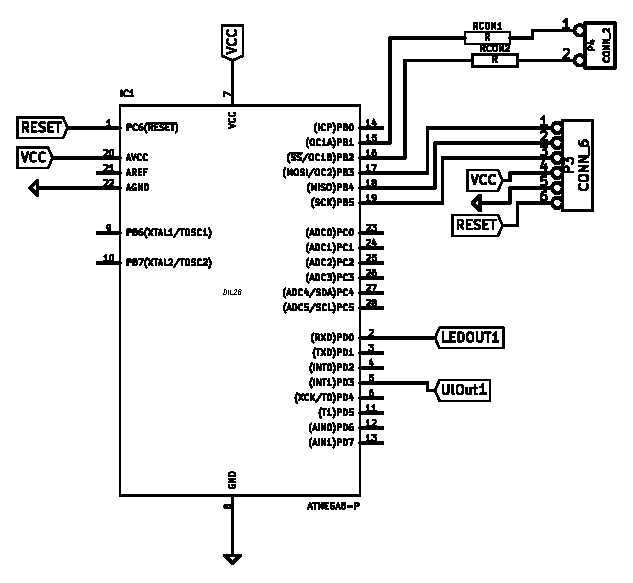
\includegraphics{Images/PWMGenerator.eps}
	\caption{PWM Signal Generator}
	\label{fig:PWMGenerator}
\end{figure}

The generated \gls{pwm} signal is fed to the Ultrasonic Transmitter, but signal sinking causes the signal to die out in the ultrasonic transmitter. So we have used a transistor to decouple the circuit from the ultrasonic transmitter. Figure.\ref{fig:Transmitter} shows the Ultrasonic transmitter attached to the output pin of \gls{pwm} generator in Atmega8.
\begin{figure}
	\centering
	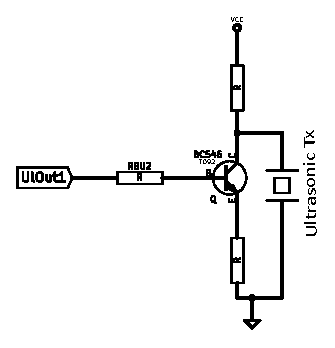
\includegraphics{Images/Transmitter.eps}
	\caption{Ultrasonic transmitter driven by \gls{pwm}}
	\label{fig:Transmitter}
\end{figure}

Also for synchronization process \gls{irled} is also driven by the microcontroller. Figure.\ref{fig:IRLEDCircuit} shows the \gls{irled} attached to the \gls{pwm} generator.

\begin{figure}
	\centering
	
\includegraphics{Images/IRLEDCircuit.eps}
	\caption{\gls{irled} driven by \gls{pwm}}
	\label{fig:IRLEDCircuit}
\end{figure}

Finally a \gls{pcb} is made for the transmitter which is shown in Figure.\ref{fig:TransmitterPCB}.

\begin{figure}
	\centering
	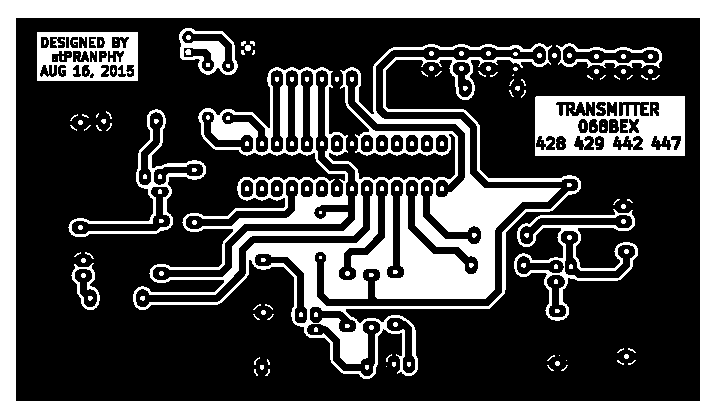
\includegraphics{Images/TransmitterPCB.eps}
	\caption{\gls{pcb} of the transmitter section}
	\label{fig:TransmitterPCB}
\end{figure}

Similarly, there are three receivers which receive the signals transmitted from transmitter section in all three directions. \gls{pcb} for the receiver is shown in Figure.\ref{fig:ReceiverPCB}
\begin{figure}[htpb]
	\centering
	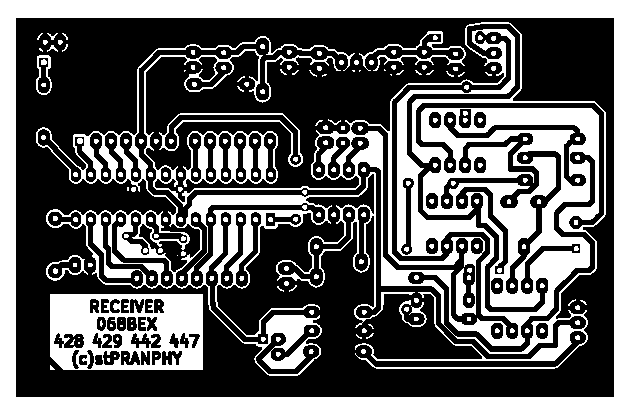
\includegraphics[scale=1]{Images/ReceiverModulePCB.eps}
	\caption{\gls{pcb} of the Receiver Module}
	\label{fig:ReceiverPCB}
\end{figure}

The receiver modules act as slave to transmit the distances to another microcontroller, which acts as a master. The implementation of master's module is as shown in Figure.\ref{fig:MasterModule}
\begin{figure}[htpb]
	\centering
	\includegraphics[scale=0.25]{Images/MasterModule.png}
	\caption{3-D view of Master Module}
	\label{fig:MasterModule}
\end{figure}
%
%
\newpage
%
\section{Components Used}

\subsection{Microcontroller ATMega8}
Atmega8 is a high-performance, Low-power AVR, 8-bit Microcontroller with advanced \gls{risc} architecture. We have used ATmega8 to generate \gls{pwm} signals, to drive \gls{irled} and Ultrasonic sensors.
\begin{figure}[h!]
	\centering
	\includegraphics[scale=0.2]{Images/Atmega8.jpg}
	\caption{Microcontroller ATMega8}
	\label{fig:ATMega8}
\end{figure}

\subsection{Operational Amplifier}
UA741 operational amplifier is used in the system. UA741 is a general purpose operational amplifier and it can be used to amplify signal in the required range 40kHz. It is stable at this frequency range and has a stable response centered at this frequency.
\begin{figure}[h!]
	\centering
	\includegraphics[scale=0.3]{Images/Opamp741.jpg}
	\caption{UA741 Operational Amplifier}
	\label{fig:Opamp741}
\end{figure}

\subsection{Tone Decoder}
IL567 Tone Decoder \gls{ic} is used in the system. This tone decoder is a general purpose tone decoder which looks for a close match between the frequency of incoming signal and of its internal oscillator. The frequency of it's internal oscillator can be controlled by adjusting the values of external capacitor and resistor connected to the IC. To filter out unnecessary signals picked up at the ultrasonic receiver we have used this IL567 Tone Decoder.
\begin{figure}[h!]
	\centering
	\includegraphics[scale=0.2]{Images/IL567.png}
	\caption{Tone Decoder IL567}
	\label{fig:IL567}
\end{figure}

\subsection{TSOP and \gls{irled}}
For the synchronization purpose we have used a pair of \gls{irled} and TSOP. \gls{irled} is used to send handshake signal which the TSOP detects and uses to synchronize the ultrasonic signal.

\begin{figure}[h!]
	\centering
	\includegraphics[scale=0.5]{Images/TSOPandIRLED.png}
	\caption{TSOP and \gls{irled}}
	\label{fig:TSOPandIRLED}
\end{figure}
%
%
\newpage
%
\section{Softwares and Tools Used}

\subsection{KiCad}
KiCad has been extensively used to design the \gls{pcb} for the circuit. We have used KiCad with the following specification.
\begin{itemize}
\item[~]Version: (25-Oct-2014 BZR 4029)-stable
\item[~]Build: wxWidgets 3.0.2 (debug,wchar\_t,compiler with C++ ABI 1002,GCC 4.9.2,wx containers,compatible with 2.8)
\item[~]Platform: Linux 3.19.0-22-generic x86\_64, 64 bit, Little endian, wxGTK
Boost version: 1.53.0
\end{itemize}

\subsection{Proteus}
Proteus is a simulation software for various designs. It is a handy tool to test programs and embedded electronics designs. It can be used to simulate programs for microcontroller as well as  test various circuits before implementing them into hardware. We have used Proteas 7.8 for the most part.

\subsection{Programmer}
Avrdude has been used as a tool to communicate between program written in computer and the microcontroller on which the program is to be written. The programmer is made form ATMEGA8 microcontroller. We opted to get one already available in the market.
\begin{figure}[h]
	\centering
	\includegraphics[scale=0.18]{Images/Programmer.jpg}
	\caption{USBasp Programmer}
	\label{fig:Programmer}
\end{figure}


\subsection{AVR GCC compiler}
AVR-GCC is a compiler that takes C language high level code and creates a binary source which can be uploaded into an AVR micro controller. Once code in 'C' is written for a particular project, AVR-GCC will turn C code into assembly language files. 

Individual assembler files are then converted into object files. Object files are files of code that AVR chips could run. The linker AVR-ld will take all these assembler files, and cross-reference functions names to create one single object file. The linker will also take modules from the 'C' library and make them into a single object. Normally this linked object is in ELF format and furthermore AVR-objcopy is used to generate a HEX format file.

%
%
\newpage
%	
%\section{Overall Circuit Description}

\subsection{Transmitter Section}

\subsection{Receiver Section}
%
%
\section{Application}
Studies have suggested that use of \gls{rtls} have significantly improved\cite{Improvement} the performance wherever it has been applied. With the recent government reports indicating increased road accidents even by the licensed drivers, it is high time we went for major overhauling in the license trial system. An \gls{rtls} based automation system would work perfect for the cause, eliminating human errors, bribery and other sneaky ways people use to get license.

%
%
%
\section{Time frame}
	With limited time to complete the project, we have a rough sketch of how we commenced and planned to complete our project. As shown in Figure \ref{fig:GanttChart}, the total available time is divided into different periods and different works are and will done in the period. 


	\begin{figure}[htbp]
		\centering
		
\begin{ganttchart}[y unit title=0.4cm,
y unit chart=0.5cm,
vgrid,hgrid, 
title label anchor/.style={below=-1.6ex},
title left shift=.05,
title right shift=-.05,
title height=1,
bar/.style={fill=gray!50},
incomplete/.style={fill=white},
progress label text={},
bar height=0.7,
group right shift=0,
group top shift=.6,
group height=.3,
group peaks={}{}{.2}]{20}
%labels
\gantttitle{2014}{2}
\gantttitle{2015}{18}\\
\gantttitle{Dec}{2}
\gantttitle{Jan}{2} 
\gantttitle{Feb}{2} 
\gantttitle{March}{2} 
\gantttitle{April}{2} 
\gantttitle{May}{2} 
\gantttitle{June}{2}
\gantttitle{July}{2}
\gantttitle{Aug}{2}
\gantttitle{Sept}{2}\\
%tasks
\ganttbar[progress=100]{Concept Note}{2}{2}\\
\ganttbar[progress=100]{Submit Proposal}{2}{2}\\
\ganttbar[progress=90]{Studies}{1}{4}\\
\ganttbar[progress=95]{Collect Component}{3}{5}\\
\ganttbar[progress=100]{Measure Distance}{6}{9}\\
\ganttbar[progress=20]{Trilateration}{10}{12}\\
\ganttbar[progress=10]{Trial Automation}{13}{16}\\
\ganttbar[progress=10]{Test System}{17}{17}\\
\ganttbar[progress=30]{Documentation}{17}{18}\\
\ganttbar[progress=0]{Presentation}{19}{19}
%~ %relations 
\ganttlink{elem0}{elem1} 
\ganttlink{elem0}{elem3} 
\ganttlink{elem3}{elem4} 
\ganttlink{elem3}{elem5}
\ganttlink{elem4}{elem5} 
\ganttlink{elem2}{elem4} 
\ganttlink{elem2}{elem5} 
\ganttlink{elem5}{elem6} 
\ganttlink{elem6}{elem7} 
\end{ganttchart}


		\caption{Work Progress Gantt Chart }
		\label{fig:GanttChart}	
	\end{figure}

	In Figure \ref{fig:GanttChart} the empty white boxes represent the work yet to be done, and the half grey filled box show the work progress till date. The completely filled boxes represent the work completed. The arrows connecting the boxes represent the sequence of works to be done.
\newpage
%
%
\newpage
%
\bibliographystyle{ieeetr}
\bibliography{Bibliographies.bib}
\nocite{Ashutosh,1003.1833,IntelligentTransport,FisherTorin,PabloJavier,Yanying}
\end{document}
